%% Except where otherwise indicated this code was originally written
%% by, and continues to be maintained by, Marcel Oliver. It is released
%% into the public domain. 
%% Where otherwise indicated, code is covered by the licensing terms of
%% the original packages.
%% The above statement was added 2009/01/05 by Clea F. Rees on behalf 
%% of the author.
% \iffalse
%%
%% File ua-classes.dtx by Marcel Oliver
%%
%% Documentation can be obtained by running "latex labels.dtx"
%%
%<*dtx>
\ProvidesFile{ua-classes.dtx}
%</dtx>
%<driver>\ProvidesFile{ua-classes.drv}
%
%<*driver>
\documentclass{ltxdoc}
\begin{document}
\DocInput{ua-classes.dtx}
\end{document}
%</driver>
% \fi
%
% \title{Document Classes for \\
%        Writing Theses and Dissertations \\
%        for Submission at the University of Arizona}
% \author{Marcel Oliver}
% \date{1996/05/09}
% \maketitle
%
% \begin{abstract}
% This package provides a \LaTeXe\ document class named |ua-thesis|
% for typesetting theses and dissertations in the official format required
% by the University of Arizona.  
% Moreover, there is a fully compatible alternative document class
% |my-thesis| for private copies of the dissertation, and the respective
% title pages are available as separate packages to work with ``any''
% document class.  
% \end{abstract}
% 
%
% \section{User Documentation}
%
% \subsection{Introduction}
%
% The |ua-thesis| document class is designed to conform with the official
% requirements of the Graduate College of the University of Arizona.  It is
% based on the |report| class which comes with the standard \LaTeX\
% distribution, and all commands are upward compatible with |report|
% and to a large extend with the |amsbook| class.  In other words, any
% document which works error free in those two classes should run with
% |ua-thesis|, too.  To automatically typeset all the required information,
% a few new commands are defined, which are explained below.
%
%
% \subsection{Classes and Options}
%
% The following classes and packages are provided:
%
% \begin{description}
%
% \item[\texttt{ua-thesis}]
% The official University of Arizona thesis document class.  The |draft|
% option is a paper saver---the automatic generation of front matter pages
% other than the title page will be suppressed, and single spaced printing
% will be used throughout the document.  The |final| option activates
% ``double spaced'' layout at the required places and creates the full set
% of front matter pages.  The default is |draft|. 
%
% Note that the draft option is passed through to the underlying |report|
% class, i.e.\ thick black rules will indicate the location of overfull
% |hbox|es.
%
% The |ua-thesis| class automatically loads the |amsmath|, |amssymb| and
% |amsthm| packages which considerably improve the mathematical
% typesetting capabilities of \LaTeX.  The use of these macros is strongly
% recommended. 
%
% The default type-size in this document class is 12pt and should not be
% changed.  Subsubsections 
% produce unnumbered run-in headings which do not appear in the Table of
% Contents, therefore their use is discouraged.
%
% \item[\texttt{my-thesis}]
% An alternative to |ua-thesis| to produce private copies of your
% dissertation which don't look so reminiscent of the typewriter age.  It
% is based on the |pcms-l| document class by the American Mathematical
% Society, which was designed to typeset monographs for the Park City/IAS
% Mathematics Series.  It is similar to |amsbook|, but has a less crowded
% look.
%
% \item[\texttt{ua-title}]
% The official University of Arizona title page as a separate package.
% Useful if you want to build your own private thesis class, but want to
% use the official title page.  It redefines the |\maketitle| command and
% also provides (potentially useless) definitions for all the commands
% described in the next section.
%
% The package is neither guaranteed nor tested to work with any specific
% document class.  You have to try and see.
%
% \item[\texttt{my-title}]
% The equivalent to |ua-title|, but with the title page of the |my-thesis|
% class. 
% 
% \end{description}
% So, the first line in your dissertation file should be
% \begin{verbatim}
%   \documentclass{ua-thesis}
% \end{verbatim}
% or, for the final printout,
% \begin{verbatim}
%   \documentclass[final]{ua-thesis}
% \end{verbatim}
% If you change the document class from |ua-thesis| to |my-thesis| or vice
% versa, the 
% first \LaTeX\ run might produce error messages because the format of the
% auxiliary files (|.aux|, |.toc| etc.) is incompatible between the two.
% Type |s| or |q| to ignore all error messages and run \LaTeX\ a second
% time, or manually delete all auxiliary  
% files before changing the document class.
% 
%
% \subsection{Commands for Specifying the Front Matter}
%
% As in the standard document classes, the title of your thesis is
% specified by
% \begin{verbatim}
%   \title{This is the Title of my Dissertation \\
%          and This is the Second Line}
% \end{verbatim}
% where line breaks can be forced with |\\| if the automatic line
% breaking does not give a satisfactory result.  But remember, the Graduate
% College imposes a maximum of three lines in the title---\LaTeX\ does not
% check this for you.  An optional argument can be given for reasons of
% compatibility with the AMS classes, but will be ignored.
%
% Your name is specified with
% \begin{verbatim}
%   \author{Firstname Lastname}
% \end{verbatim}
% again, an optional argument will be ignored.  Use
% \begin{verbatim}
%   \date{1996}
% \end{verbatim}
% set the year of your graduation.  If you omit this command, the current
% day, month and year will be printed, which may be useful for keeping
% track of different draft versions.
% The only other command that is required for the final version of every
% dissertation is 
% \begin{verbatim}
%   \director{Firstname Lastname}
% \end{verbatim}
% to specify the name of your dissertation advisor.  It will appear on the
% Special Abstract which is automatically generated.  
%
% Now the optional commands. The name of your department is set with
% \begin{verbatim}
%   \department{Department of Metaphysics}
% \end{verbatim}
% The default is ``Graduate Interdisciplinary Program in Applied
% Mathematics''. If you are in the ``Department of Metaphysics'', you have
% to use this command.
%
% If you are writing a Masters thesis, you have to explicitly specify the
% name of your degree.  Use
% \begin{verbatim}
%   \degree{Masters of Arts}
% \end{verbatim}
% The default is ``Doctor of Philosophy''.  The abbreviation of the
% degree is needed for the Special Abstract and can be with
% \begin{verbatim}
%   \degreeabbrev{M.A.}
% \end{verbatim}
% The default is ``Ph.D.''.  Moreover, for Masters theses, the Copyright
% Page will have an additional part for the approval signature of your
% advisor.  It will be automatically generated whenever you specify your
% advisor's title with
% \begin{verbatim}
%   \directortitle{Professor of Mathematics}
% \end{verbatim}
% The default is empty and \emph{must not be changed for doctoral
% dissertations}. 
%
% If you have to specify a major department
% different from the department above, use
% \begin{verbatim}
%   \major{Agriculture}
% \end{verbatim}
% The default is empty.  
%
% You can copyright your dissertation or thesis by writing
% \begin{verbatim}
%   \copyrightholder{Firstname Lastname Year}
% \end{verbatim}
% The default is empty.  If you use this command, the 
% Copyright Page will automatically change to the required
% legalese for copyrighted dissertations or theses.
% 
%
% \subsection{Examples for the Root File}
%
% For long documents such as theses, it is useful to split the \LaTeX\
% source code into several files.  The root file is the file that you run
% \LaTeX\ on.  Subordinate files are included with |\include|.
%
% \subsubsection{A Doctoral Dissertation}
%
% The example below also shows how to load the |graphics| package, which in
% particular supports the inclusion of postscript images.  Note that you
% can specify the |draft| or |final| option for the graphics package
% separate from the global options of the document class.
%
% The |ua-thesis| class is designed to create a |.dvi| file that strictly
% adheres to the required page margins.   The printer hardware or the
% driver implementation, however, may have tolerances that cause the image
% to shift on the page.  This can be corrected by using |\hoffset|
% and |\voffset|.  The example below works well with the current printers
% in the Math Department.
%
% You don't need to use |\chapter*{Dedication}| for the Dedication if you
% don't like the heading.  You can simply start a new page with |\newpage|,
% but then you are completely responsible for the formatting of that page,
% including the switch to double-spaced printing as is officially required
% (this can be done, for example, by using |\doublespaced|).
%
% \begin{verbatim}
% \documentclass[draft]{ua-thesis}
% \usepackage[final]{graphics}
%
% \hoffset -2.1mm
%
% \director{Advisor's Name}
% \date{1996}
%
% \title{This is a Doctoral Dissertation}
% \author{Your Name}
%
% \begin{document}
%
% \maketitle
%
% \chapter*{Acknowledgments}
% Acknowledgments go here.
%
% \chapter*{Dedication}
% Dedicated to the Fundamental Theorem of Calculus.
%
% \tableofcontents
% \listoffigures
% \listoftables
%
% \begin{abstract}
% This is the abstract. 
% \end{abstract}
%
% %
% Modified by Sameer Vijay
% Last Change: Tue Jul 26 2005 13:00 CEST
%
%%%%%%%%%%%%%%%%%%%%%%%%%%%%%%%%%%%%%%%%%%%%%%%%%%%%%%%%%%%%%%%%%%%%%%%%
%
% Sample Notre Dame Thesis/Dissertation
% Using Donald Peterson's ndthesis classfile
%
% Written by Jeff Squyres and Don Peterson
%
% Provided by the Information Technology Committee of
%   the Graduate Student Union
%   http://www.gsu.nd.edu/
%
% Nothing in this document is serious except the format.  :-)
%
% If you have any suggestions, comments, questions, please send e-mail
% to: ndthesis@gsu.nd.edu
%
%%%%%%%%%%%%%%%%%%%%%%%%%%%%%%%%%%%%%%%%%%%%%%%%%%%%%%%%%%%%%%%%%%%%%%%%


%
% Chapter 1
%

\chapter{INTRODUCTION}

\section{Overview}

This is an overview of the introduction.  In here, I will use many
many buzzwords and other legalistic-types of terms, mostly begining on
the expounding of the holistic and synergistic energy that Gnus bring
to our organizations.

\subsection{Background}

In preparation for reading this dissertation, I would highly recommend
reading some of the other material available on
Gnus~\citep{gnus98:_gerry_ganst,greenfield96:_gettin_know_gnu}.  They
are very well written and will give you a fuller understanding of
Gnus.

Gnus are frequently mistakes for squirrels.  They are not squirrels.
They are Gnus.  Don't call them squirrels, either (unless you have
food in your hand); they tend to get a bit upset.\footnote{This is
  frequently mistaken for the chattering and scampering away.  Gnus
  are actually quite polite; they will leave if they have nothing nice
  to say, for fear of saying something offensive.}  If you have food
in your hand, they tend to ignore this insult and accept your food as
a peace offering.

\subsection{Foreground}

Table~\ref{tbl:bogus1} shows some feeding frequencies for where Gnus
like to eat around the Notre Dame campus.  Gnus have work weeks, just
like humans do, hence the much lower frequencies on weekends.  This
can lead us to conclude that Gnu weekend shifts are much smaller than
the normal work-week shifts.  In fact, we can attempt to parametrize the
sighting frequency, $\mathcal{F}$, by the student population, type of food, and
day of the week as:
\begin{equation}
  \mathcal{F} = \mathcal{F}(p,f,d).
\end{equation}
Table~\ref{tbl:bogus2} shows what they
typically like to eat.

\begin{table}[tpb]
  \begin{center}
    \caption{WHERE Gnus LIKE TO EAT \label{tbl:bogus1}}
    \begin{tabularx}{0.85\textwidth}{lrrrrrrr} \toprule
      \multicolumn{1}{c}{Location} & Sun & Mon & Tue & Wed & Thu & Fri & Sat \\ \midrule
      Front of Dome & 1 & 5 & 6 & 5 & 4 & 5 & 1 \\
      Stonehenge & 2 & 9 & 10 & 12 & 9 & 14 & 2 \\
      The Rock & 1 & 3 & 4 & 3 & 4 & 3 & 0 \\
      The ACC & 3 & 4 & 5 & 5 & 5 & 4 & 1 \\
      Dining Halls & 5 & 14 & 12 & 13 & 14 & 12 & 3 \\
      Hesburgh Library & 2 & 3 & 5 & 2 & 3 & 4 & 2 \\ \bottomrule
    \end{tabularx}
  \end{center}
\end{table}

\begin{table}[tpb]
  \setlength{\capwidth}{0.7\textwidth}
  \begin{center}
    \caption{WHAT Gnus LIKE TO EAT ON THE NOTRE DAME CAMPUS, LISTED
      BY AVERAGE NUMBER OF SIGHTINGS PER WEEKDAY
    \label{tbl:bogus2}
}
    \begin{tabular}{lrrrrrrr} \toprule
      \multicolumn{1}{c}{Food} & Sun & Mon & Tue & Wed & Thu & Fri & Sat \\ \midrule
      Twinkies & 1 & 5 & 6 & 5 & 4 & 5 & 1 \\
      Ding Dongs & 2 & 9 & 10 & 12 & 9 & 14 & 2 \\
      Carrots & 1 & 3 & 4 & 3 & 4 & 3 & 0 \\
      Lettuce & 3 & 4 & 5 & 5 & 5 & 4 & 1 \\
      Twizlers & 5 & 14 & 12 & 13 & 14 & 12 & 3 \\
      Jawbreakers & 2 & 3 & 5 & 2 & 3 & 4 & 2 \\ \bottomrule
    \end{tabular}
  \end{center}
\end{table}

Figure~\ref{fig:bogus3} shows a nice graph of location distributions
by day of week.  I have no real reason for including it except to show
that figures work as well.  Did I mention that Gnus are really cool?

\begin{figure}[tpb]
  \begin{center}
    \centerline{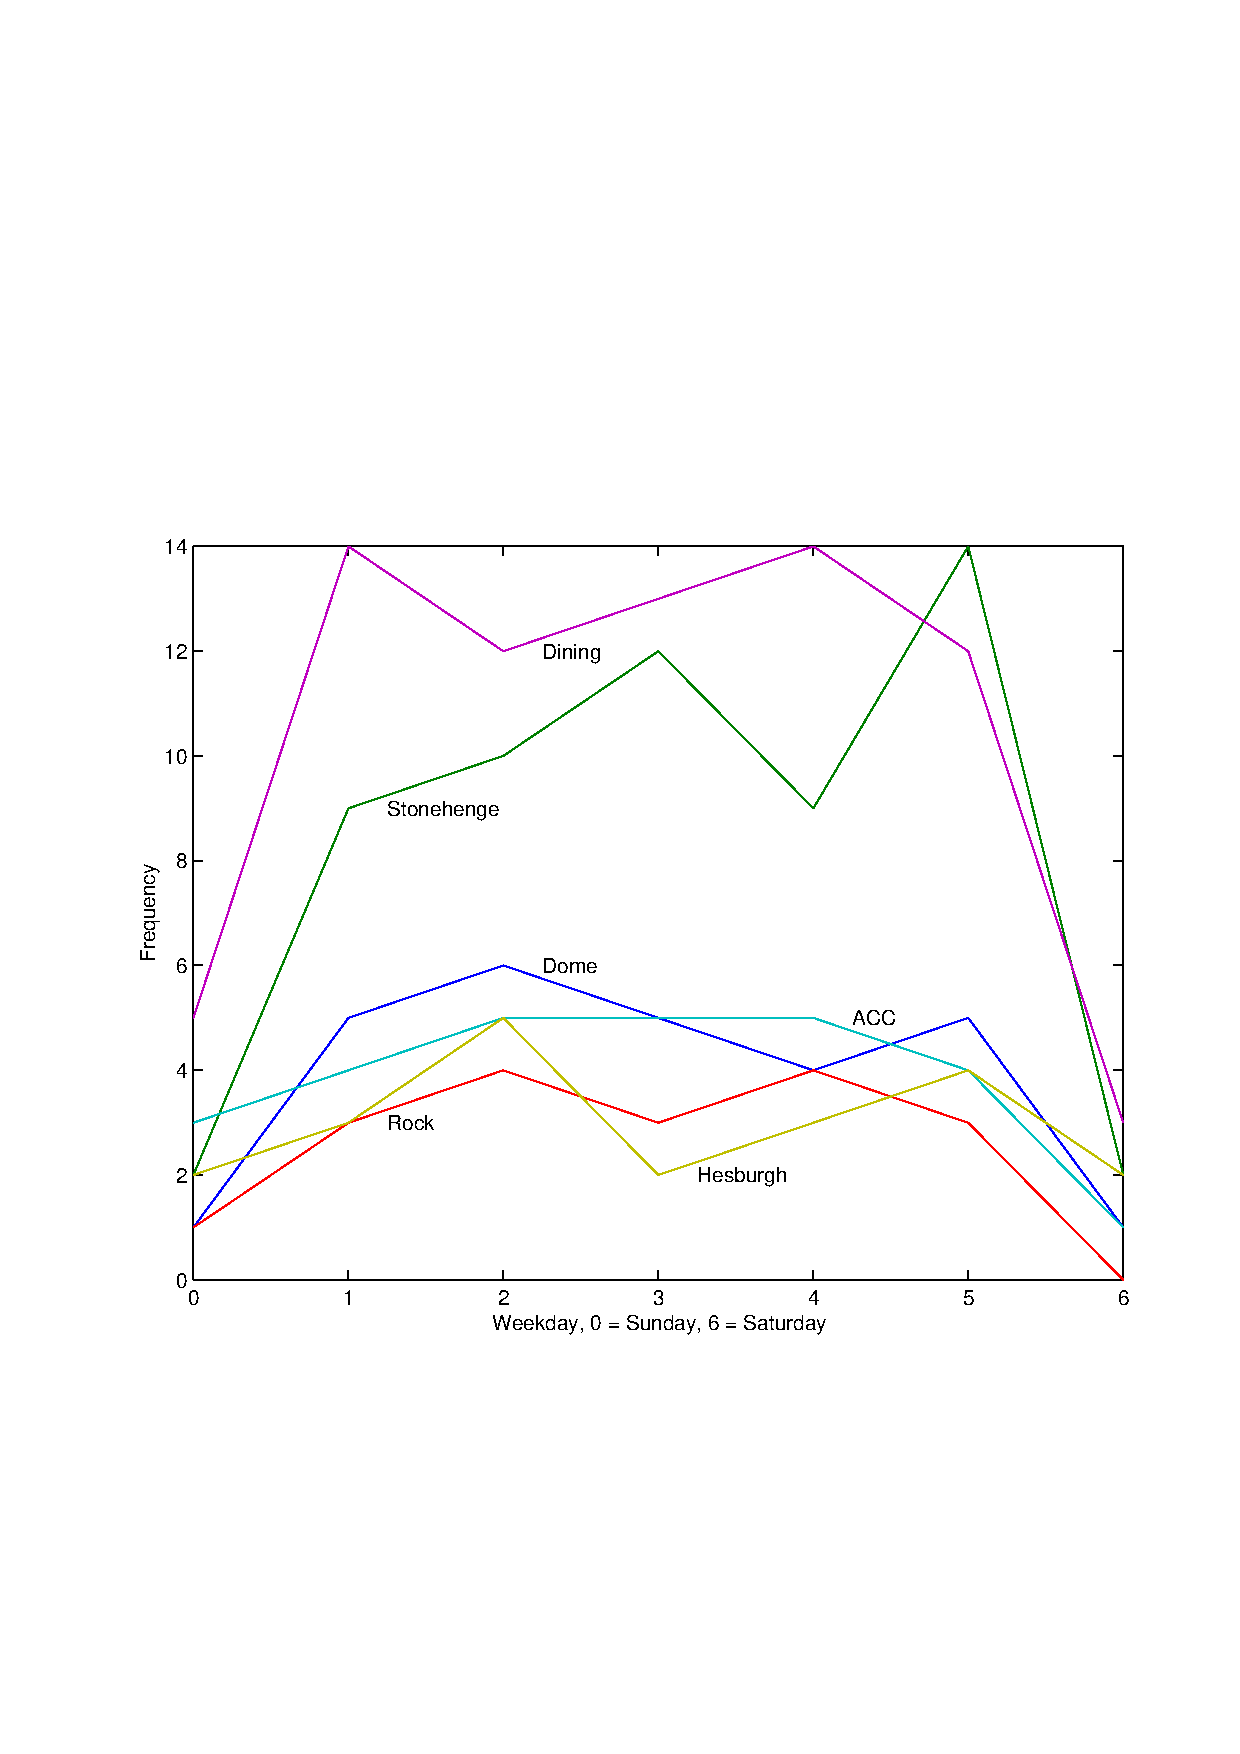
\includegraphics[scale=0.8]{sample_nd}}
    \caption{Location distributions by day of where, where the X axis
      is the weekday (0 through 6), and the Y axis is the sighting
      frequency}
    \label{fig:bogus3}
  \end{center}
\end{figure}

Gnus typically tend to come out when there are large gatherings of
humans with food.  Gnus work very hard at providing us with all the
things that we like (trees, dirt, air, etc.), and so we should freely
give them food.  They will come up and stand a respectful distance
away from you, waiting to see if they will be rewarded for their
efforts.  If you offer some food, they will take it and back off a
respectful distance in order to consume their food while leaving you
to your ``personal space.''  

\section{Groovin' Gnus}
\label{sec:groovin-gnus}

Gnus do tend to stay away from humans in their normal day-to-day
workings.  This is mainly because humans don't, for the most part,
understand what they are doing.  If a Gnu is working, and a human
approaches it, the Gnu will tend to drop whatever it is doing and run
away.  This is probably do to the tendency for humans to have ``group
meetings'' and ``productivity seminars.''  Most Gnus are deathly
afraid of such overmanagement, and run at the slightest hint of it,
for fear that it will cripple their real work.

It is interesting, however, that Gnus have chosen an Institution of
Higher Education for their BOO.\footnote{Base of Operations.}  It is
often said that:
\begin{quote}
  Academic politics are the dirtiest, meanest, ugliest, and generally
  the most low-down, in-your-face, and kick-em-while-they're-down than
  anywhere else (even Washington D.C.)  because the stakes are so low.
\end{quote}
It has been hypothesized that the Gnus are subtly trying to affect a
change for the better (i.e., eliminating the overmanagement problems)
by working the very system that they are trying to change, from
within.  That is, the graduates from Notre Dame can learn from the
examples of the Gnus here, and run screaming (or chattering) at the
slightest hint of overmanagement, and let the real work proceed
unhindered.

% % uncomment the following lines,
% if using chapter-wise bibliography
%
% \bibliographystyle{ndnatbib}
% \bibliography{example}

% \chapter{فضاهای فشرده پایدار و فضاهای مرتب فشرده}
\thispagestyle{empty}
\section{فضاهای فشرده پایدار}
یک فضای توپولوژیک جزئاً مرتب (یا به طور خلاصه، فضای مرتب)، از دیدگاه آبرامسکی
\cite{abramsky2}،
مجموعه‌ای مانند $ X $ همراه 
با یک توپولوژی $ \mathcal{O} $ و یک ترتیب $ \leq $ است به طوری که گراف ترتیب در $X\times X  $ بسته باشد. بنابراین ...
\section{فضاهای مرتب فشرده}
در این  بخش به بیان ...
% \appendix
% %% Proposal appendix


%
% \begin{thebibliography}{99}
% And the bibliography goes here.  
% \end{thebibliography}
%
% \end{document}  
% \end{verbatim}
%
% \subsubsection{A Masters Thesis}
%
% This thesis is copyrighted, but does not have Acknowledgments or a
% Dedication.  It is written by a student in the Department of
% Mathematics. 
%
% \begin{verbatim}
% \documentclass[final]{ua-thesis}
%
% \hoffset -2.1mm
%
% \director{Advisor's Name}
% \directortitle{Professor of Mathematics}
% \degree{Master of Science}
% \degreeabbrev{M.S.}
% \department{Department of Mathematics}
% \date{1996}
%
% \title{This is a Masters Thesis}
% \author{Your Name}
% \copyrightholder{Your Name 1996}
%
% \begin{document}
%
% \maketitle
% \tableofcontents
% \listoffigures
% \listoftables
%
% \begin{abstract}
% This is the abstract. 
% \end{abstract}
%
% %
% Modified by Sameer Vijay
% Last Change: Tue Jul 26 2005 13:00 CEST
%
%%%%%%%%%%%%%%%%%%%%%%%%%%%%%%%%%%%%%%%%%%%%%%%%%%%%%%%%%%%%%%%%%%%%%%%%
%
% Sample Notre Dame Thesis/Dissertation
% Using Donald Peterson's ndthesis classfile
%
% Written by Jeff Squyres and Don Peterson
%
% Provided by the Information Technology Committee of
%   the Graduate Student Union
%   http://www.gsu.nd.edu/
%
% Nothing in this document is serious except the format.  :-)
%
% If you have any suggestions, comments, questions, please send e-mail
% to: ndthesis@gsu.nd.edu
%
%%%%%%%%%%%%%%%%%%%%%%%%%%%%%%%%%%%%%%%%%%%%%%%%%%%%%%%%%%%%%%%%%%%%%%%%


%
% Chapter 1
%

\chapter{INTRODUCTION}

\section{Overview}

This is an overview of the introduction.  In here, I will use many
many buzzwords and other legalistic-types of terms, mostly begining on
the expounding of the holistic and synergistic energy that Gnus bring
to our organizations.

\subsection{Background}

In preparation for reading this dissertation, I would highly recommend
reading some of the other material available on
Gnus~\citep{gnus98:_gerry_ganst,greenfield96:_gettin_know_gnu}.  They
are very well written and will give you a fuller understanding of
Gnus.

Gnus are frequently mistakes for squirrels.  They are not squirrels.
They are Gnus.  Don't call them squirrels, either (unless you have
food in your hand); they tend to get a bit upset.\footnote{This is
  frequently mistaken for the chattering and scampering away.  Gnus
  are actually quite polite; they will leave if they have nothing nice
  to say, for fear of saying something offensive.}  If you have food
in your hand, they tend to ignore this insult and accept your food as
a peace offering.

\subsection{Foreground}

Table~\ref{tbl:bogus1} shows some feeding frequencies for where Gnus
like to eat around the Notre Dame campus.  Gnus have work weeks, just
like humans do, hence the much lower frequencies on weekends.  This
can lead us to conclude that Gnu weekend shifts are much smaller than
the normal work-week shifts.  In fact, we can attempt to parametrize the
sighting frequency, $\mathcal{F}$, by the student population, type of food, and
day of the week as:
\begin{equation}
  \mathcal{F} = \mathcal{F}(p,f,d).
\end{equation}
Table~\ref{tbl:bogus2} shows what they
typically like to eat.

\begin{table}[tpb]
  \begin{center}
    \caption{WHERE Gnus LIKE TO EAT \label{tbl:bogus1}}
    \begin{tabularx}{0.85\textwidth}{lrrrrrrr} \toprule
      \multicolumn{1}{c}{Location} & Sun & Mon & Tue & Wed & Thu & Fri & Sat \\ \midrule
      Front of Dome & 1 & 5 & 6 & 5 & 4 & 5 & 1 \\
      Stonehenge & 2 & 9 & 10 & 12 & 9 & 14 & 2 \\
      The Rock & 1 & 3 & 4 & 3 & 4 & 3 & 0 \\
      The ACC & 3 & 4 & 5 & 5 & 5 & 4 & 1 \\
      Dining Halls & 5 & 14 & 12 & 13 & 14 & 12 & 3 \\
      Hesburgh Library & 2 & 3 & 5 & 2 & 3 & 4 & 2 \\ \bottomrule
    \end{tabularx}
  \end{center}
\end{table}

\begin{table}[tpb]
  \setlength{\capwidth}{0.7\textwidth}
  \begin{center}
    \caption{WHAT Gnus LIKE TO EAT ON THE NOTRE DAME CAMPUS, LISTED
      BY AVERAGE NUMBER OF SIGHTINGS PER WEEKDAY
    \label{tbl:bogus2}
}
    \begin{tabular}{lrrrrrrr} \toprule
      \multicolumn{1}{c}{Food} & Sun & Mon & Tue & Wed & Thu & Fri & Sat \\ \midrule
      Twinkies & 1 & 5 & 6 & 5 & 4 & 5 & 1 \\
      Ding Dongs & 2 & 9 & 10 & 12 & 9 & 14 & 2 \\
      Carrots & 1 & 3 & 4 & 3 & 4 & 3 & 0 \\
      Lettuce & 3 & 4 & 5 & 5 & 5 & 4 & 1 \\
      Twizlers & 5 & 14 & 12 & 13 & 14 & 12 & 3 \\
      Jawbreakers & 2 & 3 & 5 & 2 & 3 & 4 & 2 \\ \bottomrule
    \end{tabular}
  \end{center}
\end{table}

Figure~\ref{fig:bogus3} shows a nice graph of location distributions
by day of week.  I have no real reason for including it except to show
that figures work as well.  Did I mention that Gnus are really cool?

\begin{figure}[tpb]
  \begin{center}
    \centerline{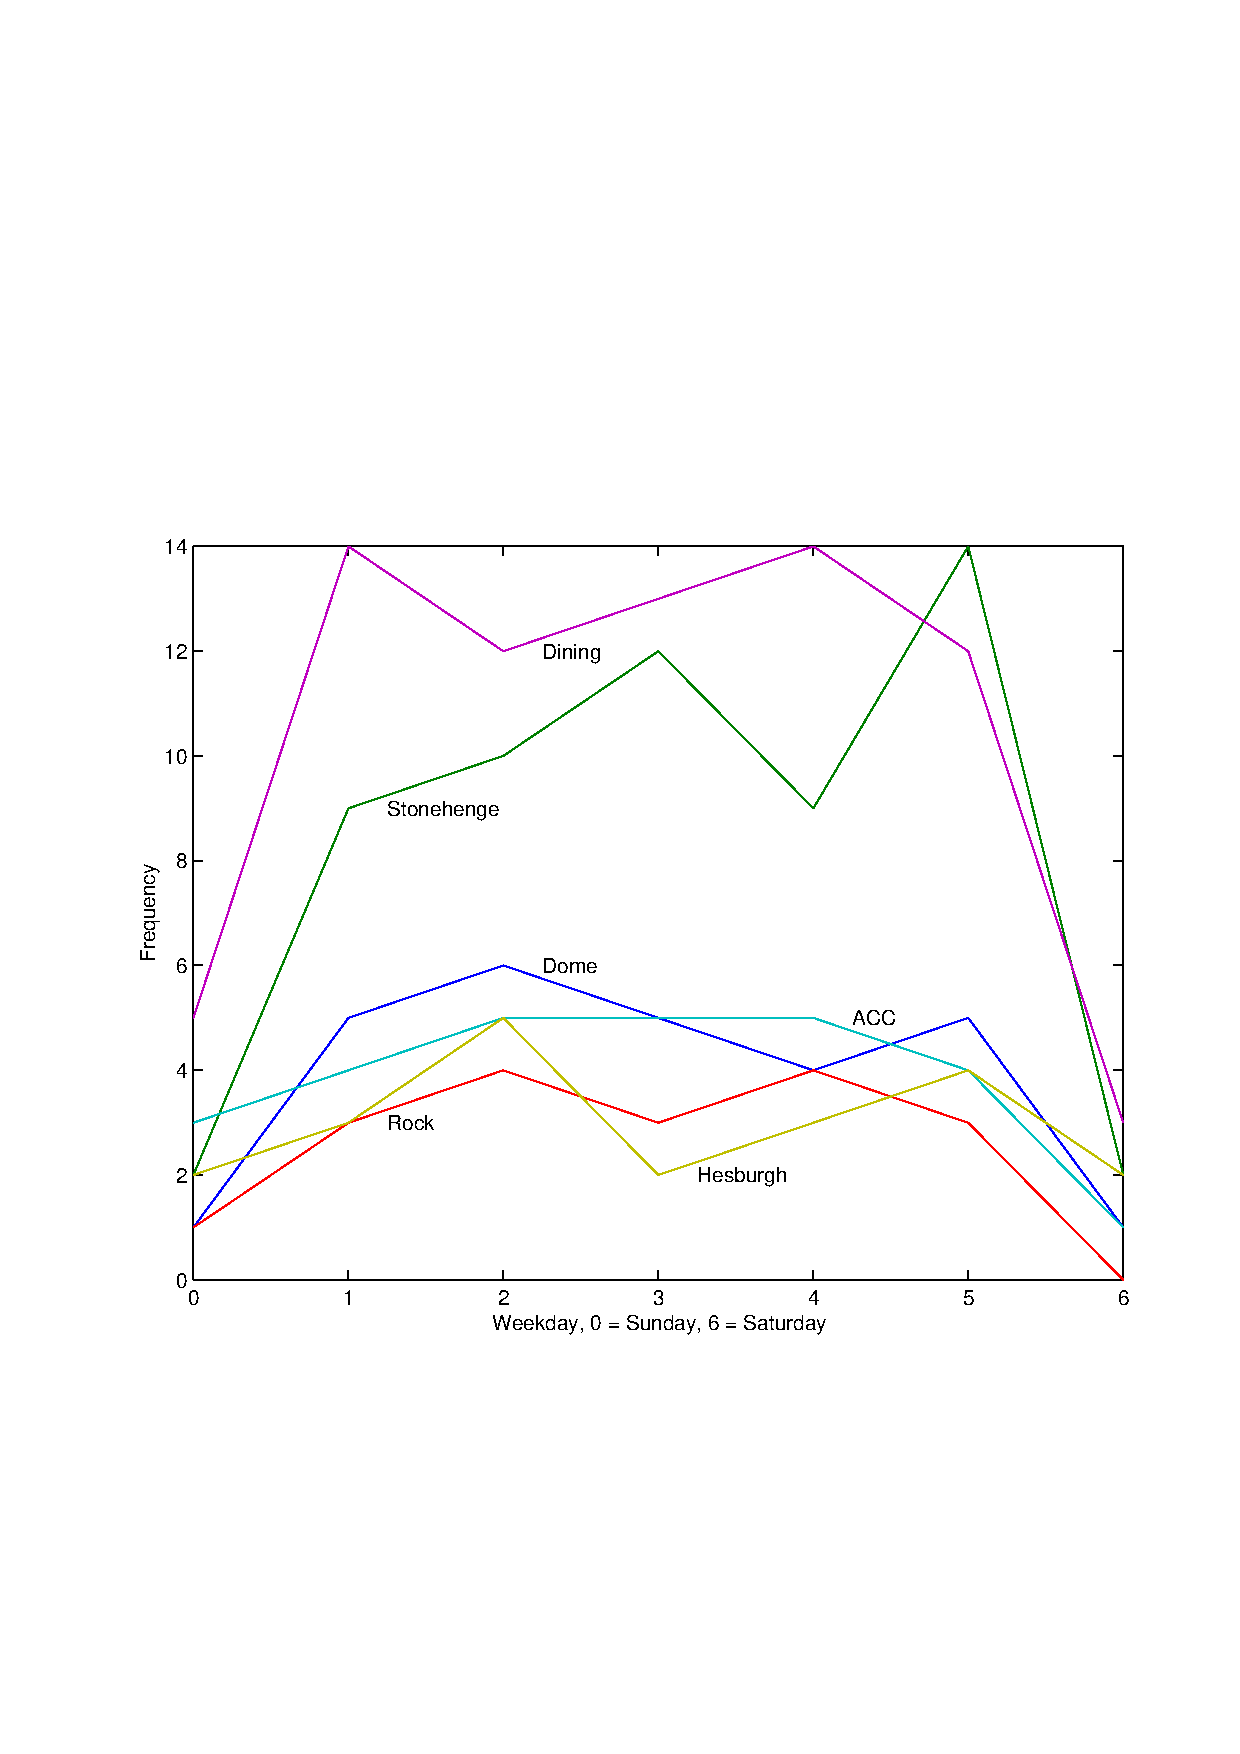
\includegraphics[scale=0.8]{sample_nd}}
    \caption{Location distributions by day of where, where the X axis
      is the weekday (0 through 6), and the Y axis is the sighting
      frequency}
    \label{fig:bogus3}
  \end{center}
\end{figure}

Gnus typically tend to come out when there are large gatherings of
humans with food.  Gnus work very hard at providing us with all the
things that we like (trees, dirt, air, etc.), and so we should freely
give them food.  They will come up and stand a respectful distance
away from you, waiting to see if they will be rewarded for their
efforts.  If you offer some food, they will take it and back off a
respectful distance in order to consume their food while leaving you
to your ``personal space.''  

\section{Groovin' Gnus}
\label{sec:groovin-gnus}

Gnus do tend to stay away from humans in their normal day-to-day
workings.  This is mainly because humans don't, for the most part,
understand what they are doing.  If a Gnu is working, and a human
approaches it, the Gnu will tend to drop whatever it is doing and run
away.  This is probably do to the tendency for humans to have ``group
meetings'' and ``productivity seminars.''  Most Gnus are deathly
afraid of such overmanagement, and run at the slightest hint of it,
for fear that it will cripple their real work.

It is interesting, however, that Gnus have chosen an Institution of
Higher Education for their BOO.\footnote{Base of Operations.}  It is
often said that:
\begin{quote}
  Academic politics are the dirtiest, meanest, ugliest, and generally
  the most low-down, in-your-face, and kick-em-while-they're-down than
  anywhere else (even Washington D.C.)  because the stakes are so low.
\end{quote}
It has been hypothesized that the Gnus are subtly trying to affect a
change for the better (i.e., eliminating the overmanagement problems)
by working the very system that they are trying to change, from
within.  That is, the graduates from Notre Dame can learn from the
examples of the Gnus here, and run screaming (or chattering) at the
slightest hint of overmanagement, and let the real work proceed
unhindered.

% % uncomment the following lines,
% if using chapter-wise bibliography
%
% \bibliographystyle{ndnatbib}
% \bibliography{example}

% \chapter{فضاهای فشرده پایدار و فضاهای مرتب فشرده}
\thispagestyle{empty}
\section{فضاهای فشرده پایدار}
یک فضای توپولوژیک جزئاً مرتب (یا به طور خلاصه، فضای مرتب)، از دیدگاه آبرامسکی
\cite{abramsky2}،
مجموعه‌ای مانند $ X $ همراه 
با یک توپولوژی $ \mathcal{O} $ و یک ترتیب $ \leq $ است به طوری که گراف ترتیب در $X\times X  $ بسته باشد. بنابراین ...
\section{فضاهای مرتب فشرده}
در این  بخش به بیان ...
% \appendix
% %% Proposal appendix


%
% \begin{thebibliography}{99}
% And the bibliography goes here.  
% \end{thebibliography}
%
% \end{document}  
% \end{verbatim}
%
% \subsection{The Files and Further Documentation}
%
% Currently, the sources and all documentation are contained in the
% following three files.
% \begin{description}
%
% \item[\texttt{ua-classes.dtx}]
% User guide and documented source code.  The document you are reading has
% been obtained by running |latex ua-classes.dtx|. 
%
% \item[\texttt{ua-classes.ins}]
% The installation file. Running |latex ua-classes.ins| will 
% generate the class  files |ua-thesis.cls| and  |my-thesis.cls| as well
% as the title page packages
% |ua-title.sty| and |my-title.sty| from the universal source file
% |ua-classes.dtx|.
%
% \item[\texttt{ua-example.tex}]
% An example dissertation generated from the official Manual for Theses and
% Dissertations by the Graduate College.  The file has been obtained via
% the web and manually converted into \LaTeX.  It both serves as an example
% and contains the official formating instructions as of May 1996.  Be sure
% to check for changes before you submit your dissertation. 
%
% \end{description}
%
%
% \subsection{Bugs and Changes}
%
% All changes and bug fixes must be done in the file |ua-classes.dtx|,
% and \emph{not} in the files generated by the docstrip utility.  Moreover,
% they must be clearly annotated with a date, name and comments explaining
% each change.
%
%
% \section{The Code}
%
% This section contains a commented listing of the source code.
% It is intended for \TeX perts to facilitate alterations and
% debugging (hopefully the latter will not become necessary).
% 
% \subsection{The Identification Part}
%
%    \begin{macrocode}
\NeedsTeXFormat{LaTeX2e}
%<*ua-thesis>
\ProvidesClass{ua-thesis}
              [1997/03/08 UA Thesis Class]
%</ua-thesis>
%<*my-thesis>              
\ProvidesClass{my-thesis}
              [1997/03/08 My Private Thesis Class]
%</my-thesis>
%<*ua-title>
\ProvidesPackage{ua-title}[1997/03/08]
%</ua-title>
%<*my-title>
\ProvidesPackage{my-title}[1997/03/08]
%</my-title>
%    \end{macrocode}
%
% \subsection{Package Options}
%
% We pass the global package options through to the underlying
% document class.  In the |ua-thesis| class we also keep track of
% whether the |draft| or |final| option is switched on because
% we will link certain document features (see Section 1) to
% this option.
%    \begin{macrocode}
%<*ua-thesis>
\newif\iffinal@
\DeclareOption{final}{%
  \final@true
  \PassOptionsToClass{final}{report}}
\DeclareOption{draft}{%
  \final@false
  \PassOptionsToClass{draft}{report}}
\ExecuteOptions{draft}  
\DeclareOption*{\PassOptionsToClass{\CurrentOption}{report}}
\ProcessOptions
%</ua-thesis>
%    \end{macrocode}
% In the |my-thesis| class, nothing particular happens.
%    \begin{macrocode}
%<*my-thesis>
\DeclareOption*{\PassOptionsToClass{\CurrentOption}{amsbook}}
\ProcessOptions
%</my-thesis>
%    \end{macrocode}
%
% \subsection{The Underlying Document Classes}
%
% The official |ua-thesis| class is based on the standard |report|
% document class.  We load it with the |12pt| option as default,
% which is smallest size allowed.  We have to load the 
% packages of the AMS math bundle explicitly.
% Added 1997/3/8: In fact, even |ua-thesis| breaks with old versions
% of the AMS macros, so we add a release date to |\RequirePackage|.
%    \begin{macrocode}
%<*ua-thesis>
\LoadClass[12pt]{report}
\RequirePackage[reqno]{amsmath}[1996/10/24]
\RequirePackage{amsfonts}[1996/10/24]
\RequirePackage{amsthm}[1996/10/24]
\RequirePackage{ua-title}
%</ua-thesis>
%    \end{macrocode}
% We want the equation numbers on the right, thus the |reqno| option.
%
% The |my-thesis| class is based on the |amsbook| class
% with modifications adopted from the |pcms-l| package, also by the
% AMS.  The packages of the AMS math bundle are loaded by default from
% within |amsbook|.  Added 1996/12/05: The updated version works only
% with the new release of the AMS macros, dated 1996/10/24.
%    \begin{macrocode}
%<*my-thesis>
\LoadClass[reqno]{amsbook}[1996/10/24]
\RequirePackage{my-title}
%</my-thesis>
%    \end{macrocode}
%
% \subsection{General Style Settings for \texttt{ua-thesis}}
%
% Redefine the name of the Table of Contents and the References
% according to the Graduate College regulations.
% We also have to redefine |\listfigurename| and |\listtablename| with
% |\def| (although the names are not changed),
% otherwise they have the wrong status with respect to the \TeX
% internals |\outer| and |\long|, and the |\ifx| statements in the
% |\@chapterstar| macro won't work.
%    \begin{macrocode}
%<*ua-thesis>
\def\contentsname{Table of Contents}
\def\bibname{References}
\def\dedicationname{Dedication}
\def\listfigurename{List of Figures}
\def\listtablename{List of Tables}
%    \end{macrocode}
% Set the page margins as required by the Graduate College: Top margin is
% $1.5$in, bottom margin is $1$in, left margin is $1.5$in and the right
% margin is $1$in.  We grant an extra $0.2$in to the bottom margin to allow
% for printer tolerances and to account for characters that extend below
% the base line (e.g.\ the character ``y'').
%    \begin{macrocode}
\topmargin      0in
\headheight     \baselineskip
\headsep        0.6in
\addtolength{\headsep}{-\headheight}
\footskip       0in
\textheight     \paperheight
\addtolength{\textheight}{-2.7in}
\oddsidemargin  0.5in
\evensidemargin 0.5in
\marginparwidth 0in
\marginparsep   0in
\textwidth      \paperwidth
\addtolength{\textwidth}{-2.5in}
%    \end{macrocode}
% Macros to switch from single-spaced to double-spaced printing.
% The command |\doublespaced| takes only effect when it is used
% with the |final| option.
%    \begin{macrocode}
\def\singlespaced{\baselineskip=\normalbaselineskip}
\def\doublespaced{\iffinal@ \baselineskip=1.5\normalbaselineskip \fi}
%    \end{macrocode}
% Finally, we define the page styles as required.  As we are modifying the
% |\topskip| when typesetting chapter headings and when selecting
% page style |continued|, we save the default value and restore
% it on ``normal'' pages.
%    \begin{macrocode}
\newlength{\@topskipsave}
\@topskipsave\topskip
%    \end{macrocode}
% The page style |topright| is used on normal pages.  It puts
% the page number into the top
% header at the right margin of each page.
%    \begin{macrocode}
\def\ps@topright{%
    \let\@mkboth\@gobbletwo
    \topskip\@topskipsave
    \def\@oddhead{\normalfont\hfil\thepage}
    \let\@evenhead\@oddhead
    \def\@evenfoot{}
    \def\@oddfoot{}}
%    \end{macrocode}
% Page style |continued| is for the second and following pages of
% the Table of Contents, the List of Figures and the List of Tables.
% The macro |\@continued| contains the required heading for those
% pages, e.g.\ ``Table of Contents---Continued''.
%    \begin{macrocode}
\def\ps@continued{%
    \let\@mkboth\@gobbletwo
    \topskip 0.5in
    \def\@oddhead{\raisebox{-0.5in}{\@continued}%
                  \hfil\normalfont\thepage}
    \let\@evenhead\@oddhead
    \def\@evenfoot{}
    \def\@oddfoot{}}
%    \end{macrocode}
% The \TeX\ mechanism for starting pages is rather mysterious.  There is
% some extra space associated with the variable |\topskip|. However, it
% is not sufficient to just set |\topskip| to zero.  One moreover has to
% place a box of zero height onto the page, otherwise \TeX\ inserts extra
% vertical space, and we lose precise control over the placements
% of the layout elements.  The following macro is called whenever a
% title page (main title, chapter title, etc.) is started.
%    \begin{macrocode}
\def\@notopskip{\topskip\z@ \hrule height\z@}
%</ua-thesis>
%    \end{macrocode}
%
% \subsection{Some Style Defaults of the \texttt{my-thesis} Class}
%
% We mostly follow the defaults given by the |amsbook| class, but there
% are few things worth changing.  First we add some space between the items
% of a list---we don't have to be too stingy with vertical space.
% The next four lines are copied from |amsbook.cls| with changed definition
% for |\itemsep|.
%    \begin{macrocode}
%<*my-thesis>
\def\@listI{\leftmargin\leftmargini \parsep\z@skip
  \topsep\listisep \itemsep\topsep
  \listparindent\normalparindent}
\let\@listi\@listI
%    \end{macrocode}
% Moreover, sections are to be numbered within chapters, and we give the
% Abstract the appearance of an unnumbered chapter.
%    \begin{macrocode}
\numberwithin{section}{chapter}
\renewenvironment{abstract}%
  {\chapter*{Abstract}}{}
%    \end{macrocode}
% We must define a bibliography style to avoid an error message.
%    \begin{macrocode}  
\bibliographystyle{amsplain}
%</my-thesis>
%    \end{macrocode}
%
% \subsection{The Title Page Packages}
%
% The title page macros are put into separate files, so that they can
% be used in conjunction with other document classes, if this is
% desirable.
%
% First some common code that defines the macros for
% various layout elements in the title page(s).  The |my-thesis| class
% will not use all of them, but their definition is required anyway to
% assure compatibility with |ua-thesis|. The defaults are set as follows:
%    \begin{macrocode}
%<*ua-title|my-title>
\let\@title\@empty
\let\@author\@empty
\let\@copyright\@empty
\def\@thesis{Dissertation}
\def\@department{Graduate Interdisciplinary Program \\
                 in Applied Mathematics}
\def\@degree{Doctor of Philosophy}
\def\@degreeabbrev{Ph.D.}
\let\@major\@empty
\let\@director\@empty
\let\@directortitle\@empty
%    \end{macrocode}
% In the following, changed |\newcommand| to |\renewcommand|
% because the new release
% of the AMS classes seems to define |\copyrightholder| while the
% old release doesn't (1996/12/05).
%    \begin{macrocode}
\def\copyrightholder#1{\gdef\@copyright{#1}}
\newcommand{\thesis}         [1]{\gdef\@thesis{#1}}
\newcommand{\department}     [1]{\gdef\@department{#1}}
\newcommand{\degree}         [1]{\gdef\@degree{#1}}
\newcommand{\degreeabbrev}   [1]{\gdef\@degreeabbrev{#1}}
\newcommand{\major}          [1]{\gdef\@major{#1}}
\newcommand{\director}       [1]{\gdef\@director{#1}}
\newcommand{\directortitle}  [1]{\gdef\@directortitle{#1}}
%    \end{macrocode}
% We redefine the |\title| and |\author| commands to follow the
% AMS syntax.  The optional
% argument allowed in the AMS classes is simply ignored without
% an error message.
%    \begin{macrocode}
\renewcommand{\title} [2][]{\gdef\@title{#2}}
\renewcommand{\author}[2][]{\gdef\@author{#2}}
%</ua-title|my-title>
%    \end{macrocode}
% 
%
% \subsubsection{The Official Title Page}
% 
% This macro is largely self-explanatory \ldots
%
%    \begin{macrocode}
%<*ua-title>
\def\@SetTitlePage{%
  \thispagestyle{empty}
  \begingroup
    \centering
    \@notopskip
    \vspace*{1in}
    \begingroup
      \Large\scshape
      \addtolength{\baselineskip}{8pt}
      \@title \\
    \endgroup
    \vspace*{\stretch{1}}
    by \\[5pt]
    \@author \\
    \hrule height\z@
    \vspace*{\stretch{2}}
    \begingroup
      \rule{2in}{0.7pt} \\
      \ifx\@empty\@copyright
        \else Copyright \copyright\ \@copyright \\
        \fi
    \endgroup
    \vspace*{\stretch{2}}
    \begingroup
%    \end{macrocode}
% The following line sets the inter-word space to twice its original value.
%    \begin{macrocode}
      \spaceskip1.3\fontdimen2\font plus1.3\fontdimen3\font
      A \@thesis\ Submitted to the Faculty of the \\[8pt]
      \textsc{\large\@department} \\[8pt]
      In Partial Fulfillment of the Requirements \\
      For the Degree of \\[8pt]
      \textsc{\large\@degree}
      \ifx\@empty\@major
         \else \\
               \textsc{\large With a Major in \@major}
         \fi \\[8pt]
      In the Graduate College \\[8pt]
      \textsc{\large The University of Arizona} \\
    \endgroup
    \vspace*{\stretch{1}}
    \spaced{\@date}
    \vspace*{0.5in}
    \newpage
  \endgroup}
%    \end{macrocode}
% To make |\@SetTitlePage| work with standard document classes, we redefine
% |\maketitle| to be |\@SetTitlePage|.  This choice will later be
% overridden by the |ua-thesis| class.
%    \begin{macrocode}
\let\maketitle\@SetTitlePage
%</ua-title>
%    \end{macrocode}
%
%
% \subsubsection{My Title Page}
%
% Here we can simply redefine |\maketitle| directly without the help of
% an auxiliary macro.
%    \begin{macrocode}
%<*my-title>
\def\maketitle{%
  \cleardoublepage
  \thispagestyle{empty}
  \begingroup
    \centering
    \vspace*{\stretch{1}}
    \hrule height 1pt
    \begingroup
      \Huge\bfseries
      \addtolength{\baselineskip}{2pt}
      \medskip
      \@title \\
      \medskip
    \endgroup
    \hrule height 1pt
    \vspace*{\stretch{1}}
    \begingroup
      \huge \@author \\
    \endgroup
    \vspace*{\stretch{1.7}}
    \begingroup
      \Large
      \spaceskip1.3\fontdimen2\font plus1.3\fontdimen3\font
      A \@thesis\ Submitted to the Faculty of the \\[8pt]
      \textsc{\LARGE\@department} \\[8pt]
      In Partial Fulfillment of the Requirements \\
      For the Degree of \\[8pt]
      \textsc{\LARGE\@degree}
      \ifx\@empty\@major
         \else \\
               \textsc{\LARGE With a Major in \@major}
         \fi \\[8pt]
      In the Graduate College \\[8pt]
      \textsc{\LARGE The University of Arizona} \\
    \endgroup
    \vspace*{0.8cm}
    {\Large\spaced{\@date}}
    \newpage
  \endgroup}
%</my-title>
%    \end{macrocode}
%
%
% \subsubsection{Setting the Date with Spaces Between Digits}
% 
% In order to increase the inter-letter space in the date, we resort to
% a technique which is a simplified version of the 
% |letterspace| package (by Philip Taylor, described in The
% \LaTeX\ Companion).  The macro |\spaced| puts spaces between all the
% characters of its argument.  
%    \begin{macrocode}
%<*ua-title|my-title>
\def \spaced #1%
    {\edef \3{#1}%
     {\expandafter \insertsp@ces \3\@nd}%
    }
\def \insertsp@ces #1#2\@nd
    {\def \1{#1}%
     \def \2{#2}%
     \1%
     \ifx \1\empty \else \ifx \2\empty \else \space \fi \fi
     \ifx \2\empty
          \let \n@xt = \relax
     \else
          \futurelet \2\m@kespaceexplicit #2\@nd
          \def \n@xt {\expandafter \insertsp@ces \2\@nd}%
     \fi
     \n@xt
    }
\def \m@kespaceexplicit #1#2\@nd %
    {\if \2 \def \2{{ }#1#2}\else \def \2{#1#2}\fi}
%</ua-title|my-title>
%    \end{macrocode}
%
%
% \subsubsection{Official Approval and Copyright Pages}
%
% This code is specific to the |ua-thesis| class.  Here |\maketitle|
% has to invoke the automatic generation of the Approval and the Copyright
% Page, provided that the |final| option is set. 
%    \begin{macrocode}
%<*ua-thesis>
\def\maketitle{%
  \cleardoublepage
  \begingroup
    \@SetTitlePage
    \iffinal@
      \@SetApprovalForm
      \@SetAuthorStatement
    \fi
  \endgroup
  \let\maketitle\relax}
%    \end{macrocode}
% Make an empty approval page which is eventually to be substituted by
% the official approval page from the Graduate College.  This macro is
% only called if the |final| option is set.
%    \begin{macrocode}
\def\@SetApprovalForm{%
  \pagestyle{topright}
  \@notopskip
  \vspace*{\fill}
  \begin{center}
    \Large
    Get the official approval page \\
    from the Graduate College \\
    \textsl{before} your final defense.
  \end{center}
  \vspace*{\fill}
  \vspace*{0.5in}
  \newpage}
%    \end{macrocode}
% Now the Copyright page.  The copyright page is also printed only
% with the |final| option in place.
%    \begin{macrocode}
\def\@SetAuthorStatement{%
   \begingroup
     \pagestyle{topright}
     \@notopskip
     \vspace*{1in}
     \begingroup
       \centering\large\scshape
       Statement by Author \\
     \endgroup
     \bigskip\bigskip
     \par
     This \MakeLowercase{\@thesis} has been submitted in partial
     fulfillment of requirements for an advanced degree at The
     University of Arizona and is deposited in the University
     Library to be made available to borrowers under rules
     of the Library.
     \bigskip
     \par
     Brief quotations from this \MakeLowercase{\@thesis} are
     allowable without special permission, provided that accurate
     acknowledgment of source is made. Requests for permission for
     extended quotation from or reproduction of this manuscript in
     whole or in part may be granted by the
     \ifx\@empty\@copyright
       head of the major department or the Dean of the Graduate
       College when in his or her judgment the proposed use of
       the material is in the interests of scholarship.
       In all other instances, however,
       permission must be obtained from the author.
     \else
       copyright holder.
     \fi
     \par
     \vspace*{3\baselineskip}
     \begin{flushright}
       \scshape
       Signed: \underline{\makebox[2.5in][r]{}}
     \end{flushright}
     \vspace*{\fill}
     \ifx\@empty\@directortitle
     \else
       \begingroup
          \centering
          \large\scshape
          Approval by \@thesis\ Director
       \endgroup
       \bigskip\bigskip\par
       This \MakeLowercase{\@thesis} has been approved
       on the date shown below:
       \vspace*{3\baselineskip}\par\noindent
       \begin{minipage}[t]{0.45\textwidth}
         \begin{center}
           \underline{\makebox[\textwidth][r]{}} \\
           \@director \\
           \@directortitle
         \end{center}
       \end{minipage}%
       \hfill%
       \begin{minipage}[t]{0.45\textwidth}
         \begin{center}
           \underline{\makebox[\textwidth][r]{}} \\
           Date
         \end{center}
       \end{minipage}
     \fi
     \vspace*{0.5in}
     \newpage
   \endgroup}
%    \end{macrocode}
%
% \subsubsection{Abstract and Special Abstract}
%
% Setting the abstract in the official thesis class
% is tricky.  Since we have to typeset it twice, for
% the regular and the special abstract, and we want to keep the regular
% \LaTeX\ syntax of having an |abstract| environment, we somehow have to 
% save the body of the abstract environment for further processing.
% This is quite difficult to do in \TeX, but fortunately the |amsmath|
% package has solved this problem for us.  It defines the internal macro
% |\collect@body| which takes a single argument, namely the name of
% a macro which does the processing.  This macro is then called by
% |\collect@body|, and given the contents of the environment body as
% its argument.  We redefine these macros here, mainly for the reason that
% we want the auxiliary macros |\collect@@body|
% and |\Addto@envbody| to be defined with
% |\long\def|, so that the abstract can have more than one paragraph.
% We capitalize all macros not to interfere with the |amsmath| package
% (actually, our change would only change |amsmath|s response to
% errors, not its behavior with correct code).
%    \begin{macrocode}
\long\def\Addto@envbody#1{\@envbody\@xp{\the\@envbody#1}}
\def\Collect@body#1{%
    \@envbody{}%
    \def\process@envbody{%
        \@xp#1\@xp{\the\@envbody}%
    }%
    \@xp\let\csname\@currenvir\endcsname\Collect@@body
    \csname\@currenvir\endcsname
}
\long\def\Collect@@body#1\end#2{%
    \def\@tempa{#2}%
    \ifx\@tempa\@currenvir
        \Addto@envbody{#1}%
        \@xp\edef\csname\@currenvir\endcsname{%
            \@nx\process@envbody\@nx\end{\@tempa}%
            }%
    \else
        \Addto@envbody{#1\end{#2}}%
    \fi
    \csname\@currenvir\endcsname
}
%    \end{macrocode}
% The details of the above are explained in |amsmath.dtx|. For us it
% is mainly a convenience, and the remainder of the abstract
% macro can be coded in a very elegant way.
%    \begin{macrocode}
\renewenvironment{abstract}{%
  \Collect@body\@SetAbstract}{}
%    \end{macrocode}
% Now the macro |\@SetAbstract|, which actually does the work. First
% we typeset the regular abstract.
%    \begin{macrocode}
\long\def\@SetAbstract#1{%
  \chapter*{Abstract} 
  #1
  \clearpage
%    \end{macrocode}
% Then the special abstract. We typeset it only in the final version. Note
% that we have to save the page counter at the beginning of the special
% abstract, so that it doesn't interfere with the page numbering of the
% main document.
%    \begin{macrocode}
  \iffinal@
  \begingroup
    \clearpage
    \newcounter{s@avepageno}
    \setcounter{s@avepageno}{\value{page}}
    \setcounter{page}{1}
    \thispagestyle{empty}  
    \@notopskip
    \begingroup
      \centering
      \large\textsc
      \@title \\
      \bigskip
      \normalfont\normalsize
      \@author, \@degreeabbrev \\
      The University of Arizona, \@date \\
    \endgroup
    \bigskip
    \noindent Director: \@director \par
    \bigskip\bigskip
    #1
  \endgroup
  \clearpage
  \setcounter{page}{\value{s@avepageno}}
  \fi}  
%    \end{macrocode}
% 
%
% \subsection{The Sectioning Commands}
%
% \subsubsection{Chapter Headings in the Official Format}
%
% The |\chapter| macro is standard code.  It calls |\@chapter| for
% numbered chapters, and |\@chapterstar| for unnumbered ones.
%    \begin{macrocode}
\def\chapter{%
  \clearpage
  \global\@topnum\z@
  \@afterindentfalse
  \secdef\@chapter\@chapterstar}
%    \end{macrocode}
% For numbered chapters we do all the usual things:  Set the page style in
% case it has been modified previously, increment the chapter counter, 
% create the Table of Contents entry and add extra space into the
% List of Figures and List of Tables.
%    \begin{macrocode}
\def\@chapter[#1]#2{%
  \pagestyle{topright}
  \refstepcounter{chapter}%
  \typeout{\@chapapp \space \thechapter}
  \addcontentsline{toc}{chapter}%
    {\protect\chapterline{\@chapapp\ \thechapter}#1}
  \addtocontents{lof}{\protect\addvspace{\medskipamount}}
  \addtocontents{lot}{\protect\addvspace{\medskipamount}}
%    \end{macrocode}
% Then we typeset the chapter heading.
%    \begin{macrocode}  
  \begingroup
    \@notopskip
    \centering
    \vspace*{0.25in}
    \textbf{\@chapapp\ \thechapter} \\
    \medskip
    \Large\textsc{#2} \par
  \endgroup
  \vspace*{2\normalbaselineskip}
  \@afterheading
  \doublespaced}
%    \end{macrocode}
% Unnumbered chapters are more tricky.  Several explicitly format decisions
% have to be made to typeset all the special ``chapters'' in the
% front matter of the dissertation according to the official requirements.
%
% The following rules are implemented: The Dedication is typeset
% double-spaced.  The Table of Contents, List of Figures and List of Tables
% must be get pagestyle |continued| and be single-spaced.  In all other
% cases pagestyle |topright| is selected.
% Only those unnumbered chapters that
% come after the Table of Contents will get an entry in the Table of
% Contents.  An arbitrary unnumbered chapter that comes after the
% Table of Contents will be double-spaced, the exception is the References,
% which are single-spaced.   If an unnumbered chapter comes before the
% Table of Contents, no explicit decision between single and double-spaced
% is made.  The effect is that the Acknowledgments will be single-spaced,
% provided they are placed in the officially required order.
%    \begin{macrocode}
\def\@chapterstar#1{%
  \typeout{#1}
  \edef\1{#1}
  \ifx \dedicationname\1
       \doublespaced
  \else     
  \ifx \contentsname\1 
       \@specialhead\1
       \singlespaced
       \let\tableofcontents\relax
  \else
  \ifx \listfigurename\1
       \@specialhead\1
       \@tocentry\1
       \singlespaced
  \else
  \ifx \listtablename\1
       \@specialhead\1
       \@tocentry\1
       \singlespaced
  \else
  \pagestyle{topright}
  \ifx \tableofcontents\relax
       \@tocentry\1
       \ifx \bibname\1 \singlespaced \else \doublespaced \fi
  \fi\fi\fi\fi\fi
%    \end{macrocode}
% And this is the code to typeset the heading.
%    \begin{macrocode}  
  \begingroup
    \@notopskip
    \centering
    \Large\textsc{#1} \par
  \endgroup
  \vspace*{2\normalbaselineskip}
  \@afterheading}
%    \end{macrocode}
% The following macro creates the Table of Contents entry for unnumbered
% chapters.
%    \begin{macrocode}
\def\@tocentry#1{%
  \addcontentsline{toc}{chapter}{#1}
  \addtocontents{lof}{\protect\addvspace{\medskipamount}}
  \addtocontents{lof}{\protect\addvspace{\medskipamount}}}
%    \end{macrocode}
% And this one switches to pagestyle |continued| and defines the
% extra part of the page heading.
%    \begin{macrocode}
\def\@specialhead#1{%
  \gdef\@continued{\normalsize\scshape#1---\slshape Continued}
  \pagestyle{continued}
  \thispagestyle{topright}}
%</ua-thesis>
%    \end{macrocode}
%
% \subsubsection{Chapter Headings in the Un-Official Format}
%
% The following code for chapter headings is taken from the
% |pcms-l| class by the AMS.  It is slightly simplified
% because we don't have to deal with different ``lectures'' and
% multiple authors.
%    \begin{macrocode}
%<*my-thesis>
\def\chapter{\cleardoublepage \pagestyle{headings}%
  \setcounter{section}0\relax
  \thispagestyle{plain}%
  \global\@topnum\z@
  \@afterindentfalse \secdef\@chapter\@schapter}
%
\def\@chapter[#1]#2{\refstepcounter{chapter}%
  \ifnum \c@secnumdepth <\z@ \let\thechapter\@empty\fi
  \let\@secnumber\thechapter
  \typeout{\chaptername\space\thechapter}%
  \addcontentsline{toc}{chapter}{%
    \protect\numberline{%
      \ifx\thechapter\@empty\else\chaptername\ \thechapter.\fi}#1}%
  \chaptermark{#1}%
  \addtocontents{lof}{\protect\addvspace{10\p@}}%
  \addtocontents{lot}{\protect\addvspace{10\p@}}%
  \@makechapterhead{#2}\@afterheading}
%
\def\@schapter#1{\typeout{#1}%
  \@ifnotempty{#1}{\addcontentsline{toc}{chapter}{#1}}%
  \let\@secnumber\empty
  \chaptermark{#1}%
  \addtocontents{lof}{\protect\addvspace{10\p@}}%
  \addtocontents{lot}{\protect\addvspace{10\p@}}%
  \@makeschapterhead{#1}\@afterheading}
%    \end{macrocode}
% For typesetting the chapter head we fixed one problem with
% |pcms-l|:  The first |\vspace| was originally achieved
% through modifying |\topskip|.  However, for mysterious reasons,
% the modification is reset to the default whenever floats are defined
% on the first page of a chapter.
%    \begin{macrocode}
\def\@makechapterhead#1{\begingroup 
  \vspace*{37pt}
   \ifodd\c@page\raggedleft\else\raggedright\fi
    \ifnum\c@secnumdepth>\m@ne
      \leavevmode
     {\Large\bfseries
              \uppercase\@xp{\chaptername}\enspace
        {\LARGE\bfseries\thechapter\par}}\skip@34\p@ 
                \advance\skip@-\normalbaselineskip
        \vskip\skip@ {\huge\bfseries #1\par}\fi
 \endgroup
  \skip@34\p@ \advance\skip@-\normalbaselineskip
  \vskip\skip@ }
%    \end{macrocode}
% And the chapter head for unnumbered chapters:
%    \begin{macrocode}
%
\def\@makeschapterhead#1{%
        \vtop to 8pc{\vfill
  \ifodd\c@page\raggedleft\else\raggedright\fi
  {\huge\bfseries #1\par}%
}%\endgroup
\skip@34\p@\advance\skip@-\normalbaselineskip
  \vskip\skip@ }
%</my-thesis>  
%    \end{macrocode}
%
% \subsubsection{Section, Subsections etc.}
%
% Here we follow literally the |pcms-l| settings, both for |ua-thesis| and
% |my-thesis|.  The appearance is similar to the |report| class, but the
% type sizes are scaled down one step, which looks less excessive.
%    \begin{macrocode}
%<*ua-thesis|my-thesis>
\def\section{\@startsection{section}{1}%
  \z@{-1\baselineskip\@plus-.75\baselineskip}{.5\baselineskip}%
  {\large\bfseries}}
%
\def\subsection{\@startsection{subsection}{2}%
  \z@{-.75\baselineskip\@plus-.5\baselineskip}{.5\baselineskip}%
  {\normalfont\bfseries}}
%
\def\subsubsection{\@startsection{subsubsection}{3}%
   \z@{.5\baselineskip\@plus.5\baselineskip}{-5\p@}%
   {\normalfont\itshape}}
%    \end{macrocode}
% The same for the appearance of theorems, remarks, definitions and
% proofs. Directly from |pcms-l|.
%
% Changed on 1996/12/05:
% The following four macros are all
% taken from the October 1996 release from |pcms-l|, because the
% new release of |amsthm| breaks these macros.  No attempt is
% made to be compatible with the old version.
%    \begin{macrocode}
\def\th@plain{%
  \let\thm@indent\noindent
  \thm@headfont{\bfseries}% heading font bold
  \thm@notefont{\mdseries\upshape}
  \thm@preskip.5\baselineskip\@plus.2\baselineskip
                                    \@minus.2\baselineskip
  \thm@postskip\thm@preskip
  \itshape
}
\def\th@remark{%
  \let\thm@indent\noindent
  \thm@headfont{\bfseries}% heading font bold
  \thm@notefont{\mdseries\upshape}%
  \thm@preskip.5\baselineskip\@plus.2\baselineskip
                                    \@minus.2\baselineskip
  \thm@postskip\thm@preskip
  \upshape
}
\def\th@definition{%
  \let\thm@indent\noindent
  \thm@headfont{\bfseries}% heading font bold
  \thm@notefont{\mdseries\upshape}%
  \thm@preskip.5\baselineskip\@plus.2\baselineskip
                                    \@minus.2\baselineskip
  \thm@postskip\thm@preskip
  \upshape
}
\renewenvironment{proof}[1][\proofname]{\par \normalfont
  \topsep6\p@\@plus6\p@ \trivlist \itemindent\z@
  \item[\hskip\labelsep\bfseries
    #1\@addpunct{.}]\ignorespaces
}{%
  \qed\endtrivlist
}
%</ua-thesis|my-thesis>
%    \end{macrocode}
%
% 
% \subsection{Captions, Headings etc.}
%
% In |ua-thesis| we redefine |\@makecaption| to change the font in captions
% for figures and tables.
%    \begin{macrocode}
%<*ua-thesis>
\long\def\@makecaption#1#2{%
  \vskip\abovecaptionskip
  \sbox\@tempboxa{\textsc{#1}. #2}%
  \ifdim \wd\@tempboxa >\hsize
    \textsc{#1}. #2\par
  \else
    \global \@minipagefalse
    \hb@xt@\hsize{\hfil\box\@tempboxa\hfil}%
  \fi
  \vskip\belowcaptionskip}
%</ua-thesis>
%    \end{macrocode}
% The corresponding changes for |my-thesis|, taken from |pcms-l|.  The
% internals work differently than with the |report| class.  Changed
% 1997/3/8: The internal font names in the |amsthm| package have
% changed with the October 1996 release.  Fixed the following two
% lines. 
%    \begin{macrocode}
%<*my-thesis>
\def\@captionheadfont{\bfseries}
\def\@captionfont{\footnotesize\mdseries}
%    \end{macrocode}
% Added 1997/3/8: We assume that both table and figure captions are
% placed below the body of the figure/table.  Thus we have to override
% amsbooks explicit assumption that table captions are placed above a
% table.  The following code is copied from |amsbook| and modified
% accordingly.
%    \begin{macrocode}
\long\def\@makecaption#1#2{%
  \setbox\@tempboxa\vbox{\color@setgroup
    \advance\hsize-2\captionindent\noindent
    \@captionfont\@captionheadfont#1\@xp\@ifnotempty\@xp
        {\@cdr#2\@nil}{.\@captionfont\upshape\enspace#2}%
    \unskip\kern-2\captionindent\par
    \global\setbox\@ne\lastbox\color@endgroup}%
  \ifhbox\@ne % the normal case
    \setbox\@ne\hbox{\unhbox\@ne\unskip\unskip\unpenalty\unkern}%
  \fi
  \ifdim\wd\@tempboxa=\z@ % this means caption will fit on one line
    \setbox\@ne\hbox to\columnwidth{\hss\kern-2\captionindent\box\@ne\hss}%
  \else % tempboxa contained more than one line
    \setbox\@ne\vbox{\unvbox\@tempboxa\parskip\z@skip
        \noindent\unhbox\@ne\advance\hsize-2\captionindent\par}%
\fi
    \addvspace\abovecaptionskip
    \moveright\captionindent\box\@ne
\relax
}
%    \end{macrocode}
% In |my-thesis| we have page headers.  Their format
% is again directly taken from the |pcms-l| class.
%    \begin{macrocode}
\def\ps@plain{\ps@empty
  \def\@oddfoot{\normalfont\footnotesize\bfseries \hfil\thepage\hfil}%
  \let\@evenfoot\@oddfoot}
\def\ps@headings{\ps@empty
  \def\@evenhead{\normalfont\footnotesize\bfseries
      \rlap{\thepage}\hfil \leftmark{}{}\hfil}%
  \def\@oddhead{\normalfont\footnotesize\bfseries \hfil
      \rightmark{}{}\hfil \llap{\thepage}}%
  \let\@mkboth\markboth
  \def\partmark{\@secmark\markboth\partrunhead\partname}%
  \def\chaptermark{%
    \@secmark\markboth\chapterrunhead{}}%
  \def\sectionmark{%
    \@secmark\markright\sectionrunhead\sectionname}%
}
%    \end{macrocode}
% Added following two lines on 1996/12/05 to have the page number on the
% second page, which is otherwise empty, appear in bold face.
%    \begin{macrocode}
\pagestyle{headings}
\chaptermark{}
\def\partrunhead#1#2#3{%
  \@ifnotempty{#2}{{#1 #2}\@ifnotempty{#3}{. }}%
  \def\@tempa{#3}%
  \ifx\@empty\@tempa\else\@tempa\fi}
\let\chapterrunhead\partrunhead
\let\sectionrunhead\partrunhead
%    \end{macrocode}
% The Bibliography style from |pcms-l|, it is less crowded than the
% original |amsbook| format.
%    \begin{macrocode}
\def\thebibliography#1{
  \chapter*\bibname
  \markboth{\bibname}{\bibname}%
  \normalsize\labelsep .5em\relax
  \list{\@arabic\c@enumi.}{\settowidth\labelwidth{\@biblabel{#1}}%
  \leftmargin\labelwidth
  \advance\leftmargin\labelsep
        \bibsetup\relax
        \usecounter{enumi}}\sloppy
  \clubpenalty9999 \widowpenalty\clubpenalty  \sfcode`\.\@m}
%    \end{macrocode}
% And, lastly, the index macro from |pcms-l|, which I haven't
% tested yet.  Let's hope it works.
%    \begin{macrocode}
\def\theindex{\cleardoublepage
\@restonecoltrue\if@twocolumn\@restonecolfalse\fi
\columnseprule \z@ \columnsep 35pt
\def\indexchap{\@startsection
                {chapter}{1}{\z@}{8pc}{34pt}%
                {\raggedright
                \huge\bfseries}}%
 \twocolumn[\indexchap*{\indexname}]
 \@mkboth{{\indexname}}{{\indexname}}%
        \thispagestyle{plain}\let\item\@idxitem\parindent\z@
         \footnotesize\parskip\z@ plus .3pt\relax\let\item\@idxitem}
%</my-thesis>
%    \end{macrocode}
% 
%
% \subsection{The Table of Contents}
%
% Modifying the design of the Table of Contents is slightly tricky.  An
% additional complication on our case is that the |amsbook| class which is
% the base for |my-thesis| considerably modifies the internals of the
% contents mechanism.  Therefore the code for the two classes is quite
% different.
%
% \subsubsection{The Official Table of Contents}
%
% At the beginning of the Document we compute the width of the boldfaced
% number 999 which we take as the maximum width of a page number in the
% Table of Contents.  Note that we have to use |\AtBeginDocument| to avoid
% typesetting anything in the preamble of the document as this will
% potentially interfere with packages that modify fonts.
%    \begin{macrocode}
%<*ua-thesis>
\newlength{\@auxlength}
\AtBeginDocument{%
  \settowidth{\@auxlength}{\textbf{999}}
  \renewcommand{\@pnumwidth}{\@auxlength}}
%    \end{macrocode}
% We want all section numbers to end with a period, and modify the
% definition of |\numberline| accordingly.
%    \begin{macrocode}  
\def\numberline#1{\hb@xt@\@tempdima{#1.\hfil}}
%    \end{macrocode}
% The same for chapter entries; in case the chapter heading takes more than
% one line, we set |\hangindent| to indent the second and following lines.
%    \begin{macrocode}
\def\chapterline#1{%
  \advance\hangindent\@tempdima
  \hbox{#1.\space\space\hfil}}  
%    \end{macrocode}
% The macro |\l@chapter| is called to set the Table of Contents line for a
% chapter entry.  
%    \begin{macrocode}
\renewcommand*\l@chapter[2]{%
  \addpenalty{-\@highpenalty}%
  \vskip 1.0em \@plus\p@
  \begingroup
    \advance\hangindent 1.5em
    \@dottedtocline{0}{0pt}{0pt}{\scshape #1}{\bfseries #2}
  \endgroup
  \penalty\@highpenalty}
%    \end{macrocode}
% And the corresponding macros for figures and tables.
%    \begin{macrocode}
\renewcommand*\l@figure[2]{%
  \@dottedtocline{1}{0pt}{30pt}{\textsc{Figure} #1}{#2}}
\renewcommand*\l@table[2]{%
  \@dottedtocline{1}{0pt}{30pt}{\textsc{Table} #1}{#2}}
%</ua-thesis>
%    \end{macrocode}
%
%
% \subsubsection{My Table of Contents}
%
% The |amsbook| class automatically calculates the width of the section
% numbers which go into the Table of Contents.  Therefore we must
% manually compute the amount of indentation for subsection entries and
% subsubsection headings.  This is done at the beginning of the document,
% after |amsbook| has read the number widths found in the previous
% \LaTeX\ run from the |.aux| file.
%    \begin{macrocode}
%<*my-thesis>
\newlength{\@subsectionindent}
\newlength{\@subsubsectionindent}
\AtBeginDocument{%
  \setlength{\@subsectionindent}{1pc}
  \addtolength{\@subsectionindent}{\csname r@tocindent1\endcsname}
  \setlength{\@subsubsectionindent}{\@subsectionindent}
  \addtolength{\@subsubsectionindent}{\csname r@tocindent2\endcsname}}
%    \end{macrocode}
% Now we modify some other style parameters.  We want subsections, but
% not subsubsections to into the Table of Contents.  If subsubsections
% should appear in the Table of Contents, the command
% |\setcounter{tocdepth}{4}| can be used in the preamble of the document.
% We also need to make some minor spacing modifications.
%    \begin{macrocode}
\setcounter{tocdepth}{3}
\renewcommand{\@pnumwidth}{2em}
\def\numberline#1{\hbox{#1\quad}}
%    \end{macrocode}
% Finally we change |\l@chapter| to get a boldface font for chapter
% entries, and redefine the subsection macros to use the indentation
% calculated above. 
%    \begin{macrocode}
\renewcommand*{\l@chapter}[2]{%
  \@tocline{0}{10pt plus4pt}{0pt}{1pc}{\bfseries}{#1}{\bfseries #2}}
\def\l@subsection{\@tocline{2}{0pt}{\@subsectionindent}{}{}}
\def\l@subsubsection{\@tocline{3}{0pt}{\@subsubsectionindent}{}{}}
%    \end{macrocode}
% We don't want a List of Figures or a List of Tables.
%    \begin{macrocode}
\let\listoffigures\relax
\let\listoftables\relax
%</my-thesis>
%    \end{macrocode}
%
% \Finale
\endinput
